\section*{Appendix}
\addcontentsline{toc}{section}{Appendix}

\subsection*{A. FinBERT Inference Details}
\label{app:finbert}

FinBERT inference ran on an Apple M4 GPU (MPS backend, $\approx$3 hours for 34,643 calls). Each transcript's Q\&A section is extracted via regex and chunked into 512-token segments. Scores ($p_\text{pos}$, $p_\text{neg}$, $p_\text{neu}$) are averaged over chunks weighted equally. Calls with fewer than 100 words are excluded. Figure~\ref{fig:finbert_dist} shows the score distributions: neutral sentiment dominates (mean $p_\text{neu} = 0.71$), with $p_\text{pos} = 0.24 \gg p_\text{neg} = 0.05$, consistent with the well-documented positivity bias in managerial communications.

\begin{figure}[H]
    \centering
    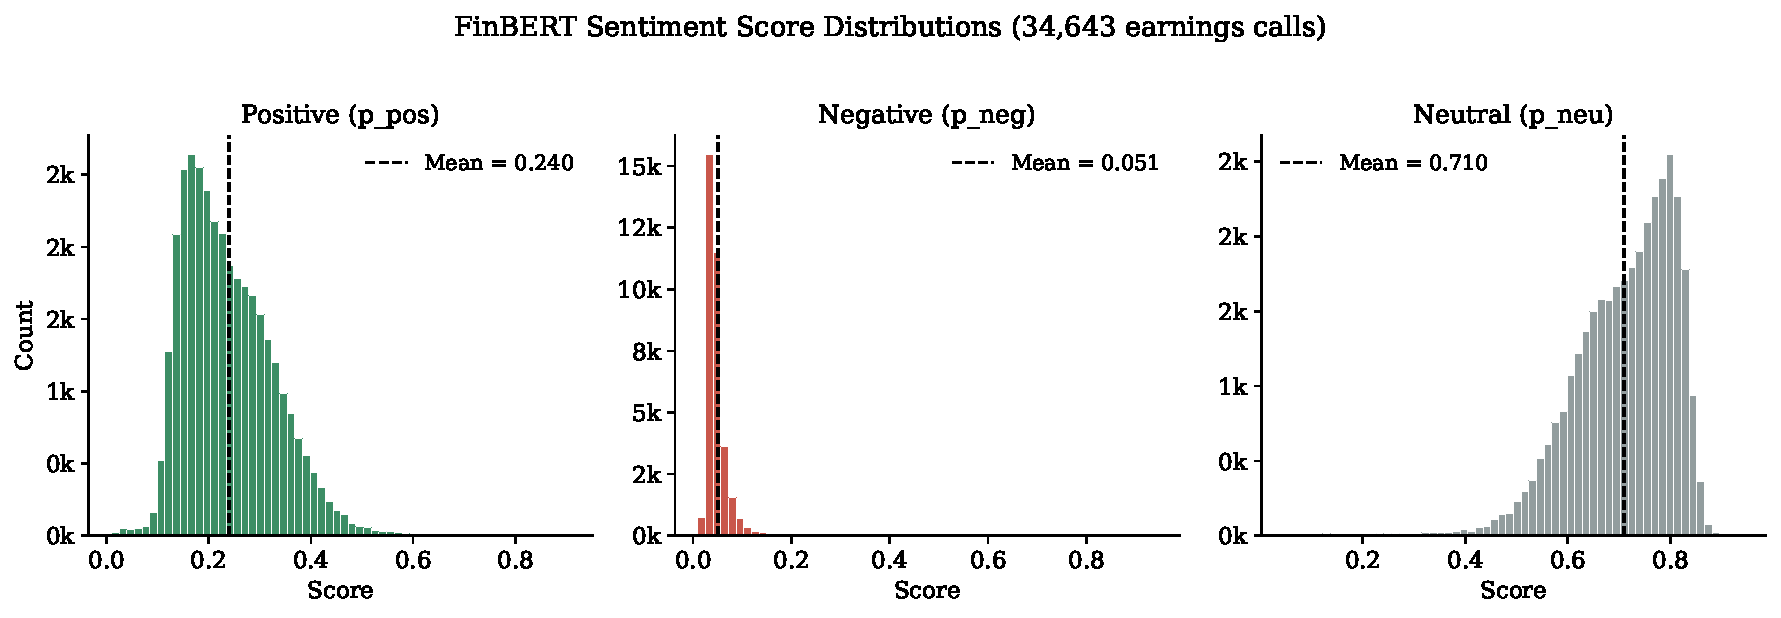
\includegraphics[width=0.85\linewidth]{figures/fig1_finbert_dist.pdf}
    \caption{FinBERT sentiment score distributions (34,643 earnings calls).}
    \label{fig:finbert_dist}
\end{figure}

\subsection*{B. Deep Learning Architecture Details}
\label{app:dl}

All DL models use Adam ($\ell_r = 10^{-3}$, weight decay $10^{-4}$, batch size 512, gradient clipping 1.0), early stopping on validation Rank IC (patience 15, max 150 epochs), and \texttt{ReduceLROnPlateau} (factor 0.5, patience 5).

\begin{enumerate}[noitemsep]
    \item \textbf{MLP\textsubscript{FinBERT}}: $12 \to 64 \to \text{BN} \to \text{ReLU} \to \text{Drop}(0.3) \to 32 \to \text{BN} \to \text{ReLU} \to \text{Drop}(0.3) \to 1$.
    \item \textbf{MLP\textsubscript{JKP+FinBERT}}: $165 \to 128 \to \text{BN} \to \text{ReLU} \to \text{Drop}(0.3) \to 64 \to \text{BN} \to \text{ReLU} \to \text{Drop}(0.3) \to 1$.
    \item \textbf{LSTM\textsubscript{FinBERT}}: $\text{LSTM}(3 \to 32, 2\,\text{layers}) \to \text{Drop}(0.3) \to \text{Linear}(32 \to 1)$. Input: last 8 quarterly call scores $(p_\text{pos}, p_\text{neg}, p_\text{neu})$, left-padded with zeros.
    \item \textbf{Attention\textsubscript{FinBERT}}: $\text{proj}(3 \to 32) + \text{PosEnc} \to 2 \times \text{EncoderLayer}(d{=}32, h{=}4, \text{ff}{=}64, \text{Pre-LN}) \to \text{MeanPool} \to \text{Linear}(32 \to 1)$. Padding mask applied; mean-pooled over non-padded positions.
\end{enumerate}

\subsection*{C. Freshness Cutoff Sensitivity}
\label{app:fresh}

\begin{table}[H]
\centering
\caption{Freshness cutoff sensitivity --- JKP + FinBERT XGBoost, out-of-sample Rank IC.}
\label{tab:freshness}
\begin{tabular}{crrrr}
\toprule
\textbf{Cutoff} & \textbf{N train} & \textbf{N test} & \textbf{Rank IC} \\
\midrule
$\leq 1$ month  & 17{,}659 & 16{,}158 & $\mathbf{0.144}$ \\
$\leq 2$ months & 29{,}153 & 26{,}378 & $0.028$ \\
$\leq 3$ months & 40{,}696 & 36{,}901 & $0.051$ \\
\bottomrule
\end{tabular}
\end{table}

The 1-month cutoff yields IC of 0.144 --- $3\times$ higher than the 3-month cutoff. The signal decays rapidly: the information advantage dissipates within 2--3 months, consistent with gradual price discovery \cite{hong2000}.

\subsection*{D. Transaction Cost Sensitivity}
\label{app:costs}

\begin{table}[H]
\centering
\caption{Transaction cost sensitivity --- LS Decile, 2019--2023.}
\label{tab:costs}
\setlength{\tabcolsep}{7pt}
\begin{tabular}{lrrrrrrrr}
\toprule
 & \multicolumn{2}{c}{\textbf{0.1\%}} & \multicolumn{2}{c}{\textbf{0.2\% (base)}} & \multicolumn{2}{c}{\textbf{0.3\%}} & \multicolumn{2}{c}{\textbf{0.4\%}} \\
\cmidrule(lr){2-3}\cmidrule(lr){4-5}\cmidrule(lr){6-7}\cmidrule(lr){8-9}
\textbf{Model} & Net & SR & Net & SR & Net & SR & Net & SR \\
\midrule
FinBERT (XGBoost)  & $+12.8\%$ & $0.88$ & $+11.4\%$ & $0.79$ & $+10.0\%$ & $0.69$ & $+8.61\%$ & $0.60$ \\
MLP\textsubscript{FinBERT} & $+9.48\%$ & $0.69$ & $+7.87\%$ & $0.58$ & $+6.26\%$ & $0.46$ & $+4.65\%$ & $0.34$ \\
\bottomrule
\end{tabular}
\end{table}

Both models remain profitable across the full cost range. FinBERT-only retains Sharpe $>0.6$ even at 0.4\% one-way.

\subsection*{E. Rolling IC and Sub-Period Analysis}
\label{app:rolling}

\begin{figure}[H]
    \centering
    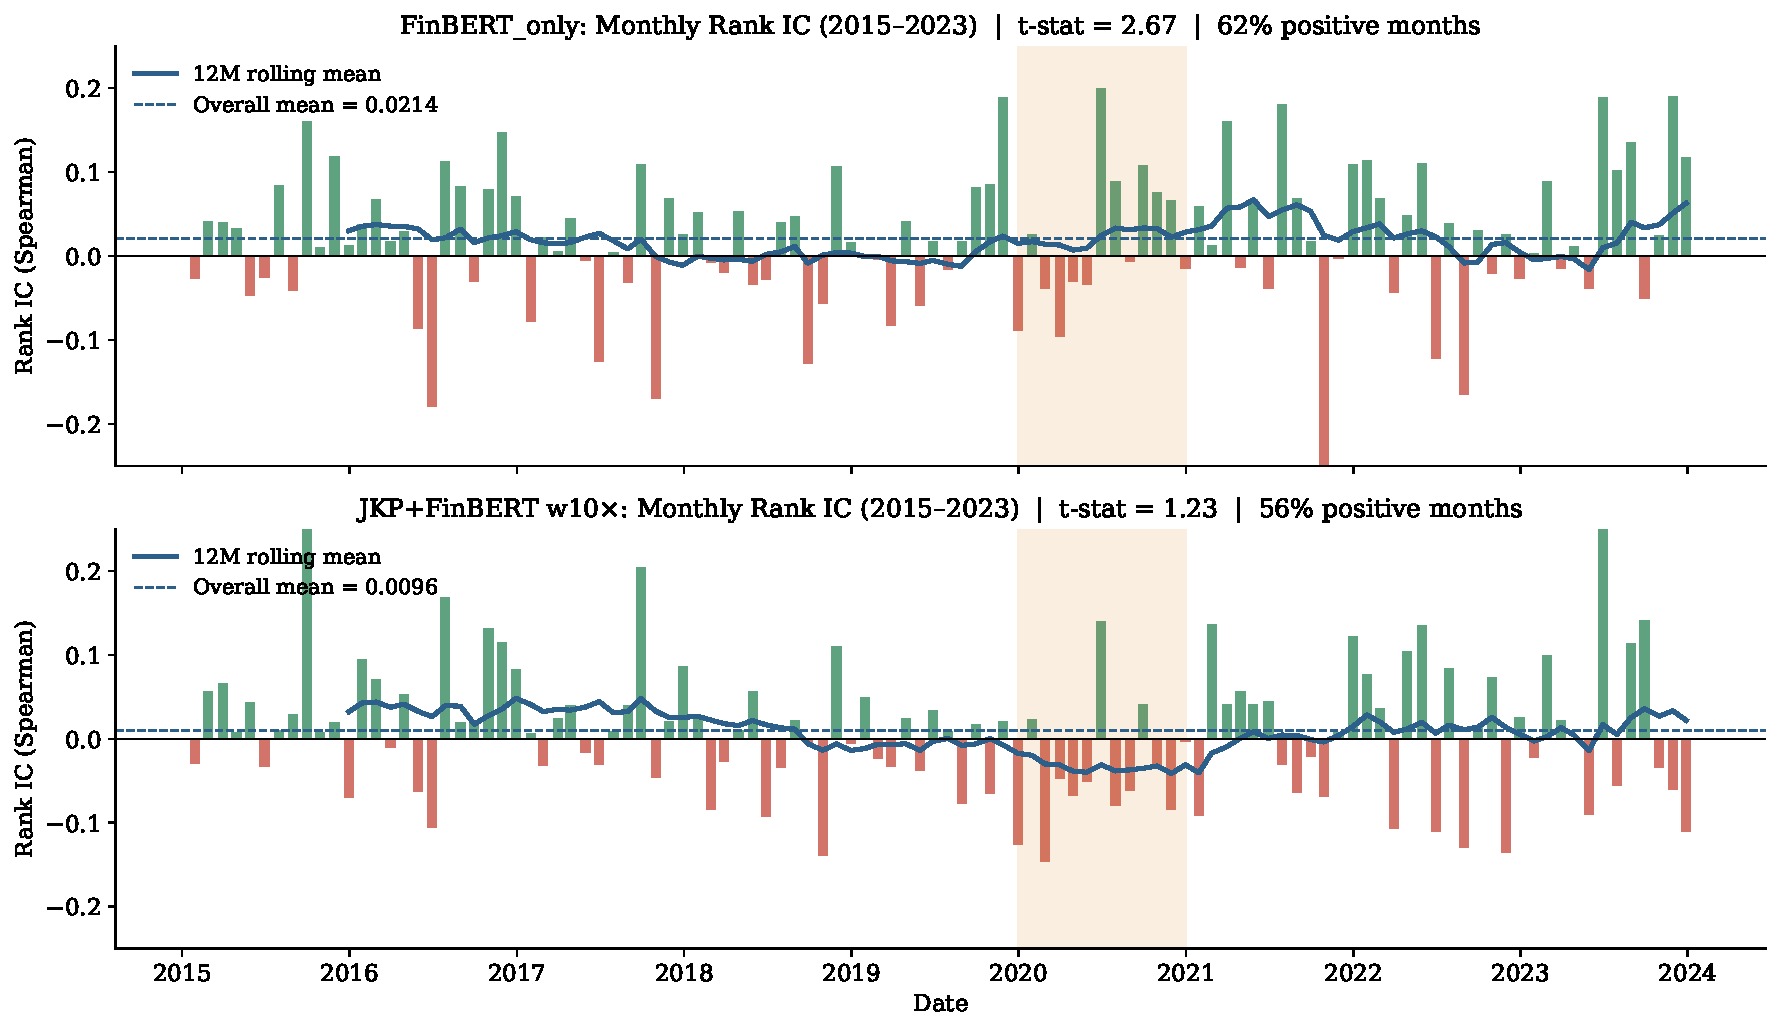
\includegraphics[width=\linewidth]{figures/fig3_monthly_ic.pdf}
    \caption{Monthly Rank IC for FinBERT-only (top) and JKP+FinBERT $\times$10 (bottom), 2015--2023.}
    \label{fig:monthly_ic}
\end{figure}

\begin{figure}[H]
    \centering
    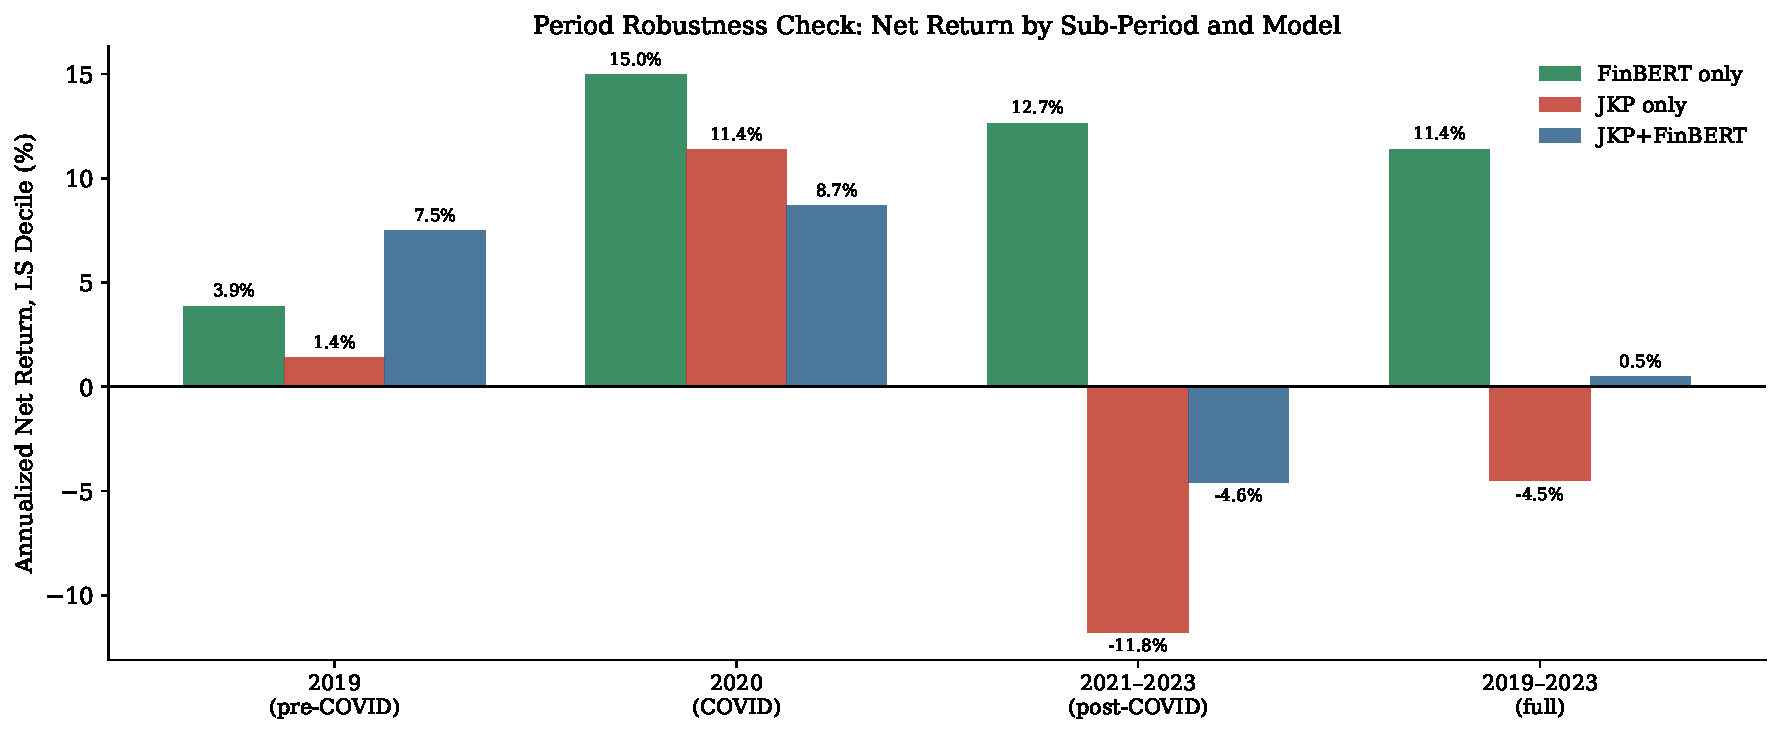
\includegraphics[width=\linewidth]{figures/fig8_period_robustness.pdf}
    \caption{Net return by sub-period. FinBERT-only is positive in all three sub-periods; its best period is 2021--2023, after the COVID-19 shock.}
    \label{fig:periods}
\end{figure}

\begin{table}[H]
\centering
\caption{FinBERT-only XGBoost LS Decile: net return and Sharpe by sub-period.}
\label{tab:periods}
\begin{tabular}{lrrl}
\toprule
\textbf{Period} & \textbf{Net} & \textbf{Sharpe} & \textbf{Remark} \\
\midrule
2019 (pre-COVID)  & $+3.87\%$ & $0.50$ & Positive in normal conditions \\
2020 (COVID-19)   & $+14.99\%$ & $0.77$ & Strong but not unique driver \\
2021--2023 (post-COVID) & $\mathbf{+12.65\%}$ & $\mathbf{0.87}$ & Best sub-period \\
2019--2023 (full) & $+11.40\%$ & $0.79$ & Full out-of-sample window \\
\bottomrule
\end{tabular}
\end{table}
